% Gemini theme
% https://github.com/anishathalye/gemini

\documentclass[final]{beamer}

% ====================
% Packages
% ====================

\usepackage[T1]{fontenc}
\usepackage{lmodern}
% \usepackage[size=custom,width=120,height=72,scale=1.0]{beamerposter}
% \usepackage[size=custom,width=172.72,height=91.44,scale=1.0]{beamerposter} % 68"x36" inches
\usepackage[size=custom,width=152.4,height=91.44,scale=1.0]{beamerposter} % 60"x36" inches
% \usepackage[size=custom,width=152.4,height=106.68,scale=1.0]{beamerposter} % 60"x42" inches
% \usepackage[size=a0]{beamerposter}
\usetheme{gemini}
% \usecolortheme{gemini}
\usecolortheme{mit}
\usepackage{graphicx}
\usepackage{booktabs}
\usepackage{tikz}
\usepackage{pgfplots}
\pgfplotsset{compat=1.14}

\usepackage{xspace}
\xspaceaddexceptions{]\{\}}
\usepackage{complexity}
\usepackage{hyperref}
\usepackage[clean]{svg}
% Tom Draper - Common LaTeX macros
%
% Requires:
% \usepackage{xspace}
% \xspaceaddexceptions{]\{\}}
% \usepackage{complexity}
%
% The LaTeX commands provided here are designed to be important in any circumstance.
% \providecommand provides the given definition if the command is not already defined.
% \ensuremath allows a command to be used in both normal and math mode.

% Include graphics from subdirectory
\graphicspath{{graphics/}}
% Since image.svg is included via \input{image.pdf_tex}, we have to add the path to \input
\makeatletter
\def\input@path{{graphics/}}
\makeatother

% Computer science words should be highlighted differently
% \providecommand{\csword}[1]{\ensuremath{\text{\tt{}#1}}\xspace}
\providecommand{\csword}[1]{\ensuremath{\text{\ComplexityFont{#1}}}\xspace}

% Math
\providecommand{\jacobi}[2]{\left( \displaystyle\frac{#1}{#2} \right)}
\providecommand{\Z}{\mathbb{Z}}
\providecommand{\Zp}{\Z/p\Z}
\providecommand{\Qbar}{\ensuremath{\overline{\mathbb{Q}}}}
% \providecommand{\gl}{\hbox{GL}_n}
% \providecommand{\floor}[1]{\left\lfloor #1 \right\rfloor}
% \providecommand{\comb}[2]{\left( {#1 \atop #2} \right)}
% \providecommand{\fract}[1]{\left\{ #1 \right\}}

% Quantum
\providecommand{\ket}[1]{\left| #1 \right\rangle}
\providecommand{\bra}[1]{\left\langle #1 \right|}
\providecommand{\braket}[2]{\left\langle #1 | #2 \right\rangle}
\providecommand{\qpic}{$\langle\textrm{q}|\textrm{pic}\rangle$\xspace}
\providecommand{\NOT}{\csword{NOT}}
\providecommand{\CNOT}{\csword{CNOT}}
\providecommand{\CCNOT}{\csword{CCNOT}}
\providecommand{\CNOTs}{\csword{CNOT}{}s\xspace}
% \providecommand{\CNOTs}{\ensuremath{\text{{\tt{}CNOT}s}}\xspace}
\providecommand{\CZ}{\csword{CZ}}
\providecommand{\CCZ}{\csword{CCZ}}
\providecommand{\XOR}{\csword{XOR}}
\providecommand{\xT}{\csword{T}}

% Complexity classes
\providecommand{\xPpoly}{\csword{P/poly}\xspace}
\providecommand{\xP}{\csword{P}}
\providecommand{\RP}{\csword{RP}}
\providecommand{\BPP}{\csword{BPP}}
\providecommand{\BQP}{\csword{BQP}}
\providecommand{\EQP}{\csword{EQP}}
\providecommand{\EQPC}{\ensuremath{\csword{EQP}_\mathbb{C}}\xspace}
\providecommand{\EQPK}{\ensuremath{\csword{EQP}_K}\xspace}
\providecommand{\EQPQ}{\ensuremath{\csword{EQP}_{\Qbar}}\xspace}
\providecommand{\QNR}{\ensuremath{\csword{QNR}}\xspace}


\providecommand{\QNR}{\csword{QNR}}
\providecommand{\QNRs}{\csword{QNR}s}
\providecommand{\ii}{\left[\jacobi{x}{17}=-1\right]}

% ====================
% Lengths
% ====================

% If you have N columns, choose \sepwidth and \colwidth such that
% (N+1)*\sepwidth + N*\colwidth = \paperwidth
\newlength{\sepwidth}
\newlength{\colwidth}
\newlength{\circwidth}
\setlength{\sepwidth}{0.025\paperwidth}
\setlength{\colwidth}{0.2\paperwidth}
\setlength{\circwidth}{0.04\paperwidth}

\newcommand{\separatorcolumn}{\begin{column}{\sepwidth}\end{column}}

% ====================
% Title
% ====================

\title{Evaluating NISQ Devices with Quadratic Nonresidues}

% \author{Thomas G. Draper \inst{1}}
\author{Thomas G. Draper}

% \institute[shortinst]{\inst{1} Center for Communications Research at La Jolla}
\institute[shortinst]{Center for Communications Research at La Jolla}

% ====================
% Footer (optional)
% ====================

\footercontent{
  \href{https://www.ccrwest.org}{https://www.ccrwest.org} \hfill
  Quantum Information Processing 2022, Pasadena, CA \hfill
  \href{mailto:tdraper@ccrwest.org}{tdraper@ccrwest.org}}
% (can be left out to remove footer)

% ====================
% Logo (optional)
% ====================

% use this to include logos on the left and/or right side of the header:
\logoleft{\includegraphics[height=4cm]{IDALogo.png}}
\logoright{\includegraphics[height=6cm]{TreeLogo}}

% \logoright{\includegraphics[height=4cm]{tree.png}\raisebox{.8cm}{\bf\Huge CCR LA JOLLA}}

% ====================
% Body
% ====================

\begin{document}

\begin{frame}[t]
% \includegraphics[width=\textwidth]{qnr17_nn.pdf}

\begin{columns}[t]
\separatorcolumn

\begin{column}{\colwidth}

  \begin{block}{An unsolved problem since Gauss}
  \begin{minipage}[c]{0.3\colwidth}
    \includegraphics[width=.25\colwidth]{gauss.jpeg}
  \end{minipage}
  \begin{minipage}[l]{0.7\colwidth}
    \heading{Quadratic nonresidue problem (\csword{QNR}):}
    \bigskip

    Given a prime $p\equiv 1\bmod 8$, find a $y$ such that $x^2\equiv y \bmod p$ has no solution.  

    \bigskip
  {\bf Question:} Is \QNR in \xP?
    \bigskip
  \end{minipage}

Gauss~\cite{gauss} proved the first nontrivial upper bound for the least quadratic nonresidue showing that $y<2\sqrt{p}+1$.
Current best analytic tools prove that $y < C\cdot p^\alpha$ for a non-zero $\alpha$~\cite[p. 33]{1993--cohen}.
  \end{block}

  \begin{exampleblock}{QNR is in \EQPC}

    {\bf We prove a new result showing a quantum computer can solve \QNR in quantum \xP.}

\begin{algorithm}
  \caption{
    % {\bf Exact quantum polynomial time algorithm for finding a quadratic nonresidues for $p\equiv 1 \bmod 8$.}
    Given $p\equiv 1 \bmod 8$, 
  choose the smallest $n$ such that $p<2^n=N$. 
    Let $\theta=\mbox{arccos}\left(1-\frac{2^n}{p-1}\right)$, and
    $f(x)=\left[\jacobi{x}{p}=-1\text{ and } 0\le x<p\right]$.
    % Let $n, N, \theta, x_0 \text{ and } f(x)$ be defined as in section~\ref{qc_alg}.
    % Let $f$ be as defined in equation~\eqref{indicator} and $\theta=\mbox{arccos}\left(1-\frac{N}{p-1}\right)$.
}
  % \label{quantum_qnr}
  \begin{noindqlist}
  \item $[O(n)]$ Apply $H^{\otimes n}$ to \( \ket{0}^{\otimes n} \) (Hadamard transform).
    \[ \frac{1}{\sqrt{N}}\sum_{x=0}^{N-1} \ket{x} \]
  \item $[O(n\log^2 n)]$ Compute Jacobi symbol indicator~\cite{harvey:hal-02070778,DBLP:journals/corr/abs-1004-2091}.
\[\frac{1}{\sqrt{N}} \sum_{x=0}^{N-1} \ket{x}\ket{\left[\jacobi{x}{p}=-1\right]}\]
\item $[O(n)]$ Compute $[x<p]$ indicator~\cite{comparator}.
\[\frac{1}{\sqrt{N}} \sum_{x=0}^{N-1} \ket{x}\ket{\left[\jacobi{x}{p}=-1\right]}\ket{[x<p]}\]
  \item $[O(1)]$ Rotate odd QNRs less than $p$ by $-2\theta$.
  % \item $[O(1)]$ Rotate odd QNRs less than $p$ by $-2\theta$, conditioned on $[x<p],\left[\jacobi{x}{p}=-1\right],$ and $x_0$.
  \[\frac{1}{\sqrt{N}} \sum_{x=0}^{N-1} e^{-i2\theta f(x)x_0}\ket{x}\ket{\left[\jacobi{x}{p}=-1\right]}\ket{[x<p]}\]
\item $[O(1)]$ Rotate all QNRs less than $p$ by $\theta$.
% \item $[O(1)]$ Rotate all QNRs less than $p$ by $\theta$, conditioned on $[x<p]$ and $\left[\jacobi{x}{p}=-1\right]$.
  \[\frac{1}{\sqrt{N}} \sum_{x=0}^{N-1} e^{i\theta f(x)(1-2x_0)}\ket{x}\ket{\left[\jacobi{x}{p}=-1\right]}\ket{[x<p]}\]
\item $[O(n\log^2 n)]$ Uncompute indicator functions.
  \[\frac{1}{\sqrt{N}} \sum_{x=0}^{N-1} e^{i\theta f(x)(1-2x_0)}\ket{x}\]
\item $[O(n)]$ Use a Grover step to invert about the mean $\alpha=\frac{1}{2\sqrt{N}}$.
    \[ \frac{1}{\sqrt N}\sum_{x=0}^{N-1} \left(1-e^{i\theta f(x) (1-2x_0)}\right)\ket{x} \]
  \item $[O(n)]$ Observe a quadratic nonresidue modulo $p$.
  \end{noindqlist}
\end{algorithm}

  \end{exampleblock}
  \begin{block}{Phase inversion in the QNR algorithm}
      \centering
    \begin{figure*}
      \includegraphics[width=.3\colwidth]{41polar_1.pdf}
    \hfill\includegraphics[width=.3\colwidth]{41polar_2.pdf}
    \hfill\includegraphics[width=.3\colwidth]{41polar_3.pdf}
      % \caption{Amplitude values for Quadratic Nonresidues for $p=41$}
      \caption{Quadratic nonresidue amplitude progression for $p=41$}
    \end{figure*}

  \end{block}

\end{column}

\separatorcolumn

\begin{column}{\colwidth}

  \begin{exampleblock}{Creating a NISQ test from the QNR algorithm}
    \heading{A quantum computer can create a probability distribution exclusively over quadratic nonresidues in polynomial time.}
    A classical algorithm capable of the same would be a mathematical breakthrough.

    Using a single Jacobi symbol calculation, a quantum computer can find a \QNR 100\% of the time, 
    whereas the classical computer success rate is bounded away from $1$. % (Probably $\frac{3}{4}$).

    % Even if we want to argue for a different classical bound, without a mathematical breakthrough,
    % the provable success rate of any algorithm in \xP will always be less than 100\%.

    \heading{The QNR algorithm evaluates two NISQ properties:}
    % Furthermore, note that the \QNR algorithm produces an equal superposition of \QNR states.
    % This allows two separate NISQ tests:
    \begin{itemize}
      \item {\bf The rate of success}
      \item {\bf The uniformity of the observations}
    \end{itemize}

    \heading{QNR Test Advantages:}
\begin{itemize}
  \item {\bf Math inspired and implementation agnostic}
  \item {\bf Infinite tests with $O(n \log^2 n)$ runtime} 
  \item {\bf Smallest tests are usable now}
  \item {\bf Scores algorithmic success instead of a physical property}
\end{itemize}
  \end{exampleblock}

  \begin{block}{General QNR algorithm}

    \begin{center}
    \begin{figure*}
      \includegraphics[width=\colwidth]{gen_alg2.pdf}
    \end{figure*}
    \end{center}

    Note than when $p=2^n+1$, the inequality indicator $[x<p]$ can be left out since there are exactly $2^n$ nonzero residues.
    Additionally, since exactly half of the values less than $2^n$ will be nonresidues, a permutation of $0,1,\ldots ,2^{n}-1$ will exist where one of the output wires is the parity bit, and another is the indicator function for the Jacobi symbol.
  This only happens for Fermat primes where $p=2^{2^m}+1$.
  \end{block}


\end{column}

\separatorcolumn

\begin{column}{\colwidth}

  \begin{block}{What can we test now?}
  \heading{Design a QNR test circuit for $p=17$}
    Since $p=17$ is a Fermat prime, the Jacobi symbol indicator is balanced.
  % For Fermat primes ($p=2^{2^n}+1$), the inequality indicator $[p<x]$ can be left out since there are exactly $2^{2^n}$ nonzero residues.

    % Additionally, a permutation of $0,1,\ldots ,2^{2^n}-1$ exists where one of the output wires is the parity bit, and another is the indicator function for the Jacobi symbol.
 $$\left[\jacobi{x}{17}=-1\right]=x_0x_1+x_0x_2+x_1x_2+x_1x_3+x_2x_3+x_0x_1x_3$$

      \heading{Jacobi symbol indicator permutation for $p=17$}
 \begin{center}
    \begin{figure*}
      \includegraphics[width=.9\colwidth]{H4_box_qnr17_indicator.pdf}
    \end{figure*}
 \end{center}

    Ideally, the Jacobi symbol circuit should be produced by an algorithm, and not by computer search.
    We accept this shortcoming in the near term, since current NISQ devices fail to escape the noise floor using the full algorithm for $p=17$.
    % This is a shortcoming of current devices, not the test itself.

    As NISQ devices improve, a full algorithmic test for $p=17$ will be preferred.
    The next tests of interest will likely be $p=41$ and $p=257$.

  \heading{Basic QNR circuit  for $p=17$}

  \begin{center}
    \begin{figure*}
      \includegraphics[width=\colwidth]{qnr17_full_circuit.pdf}
      % \caption{QNR test for $p=17$}
    \end{figure*}
  \end{center}

  \end{block}

  \begin{block}{Running the QNR17 circuit on current NISQ devices}
    Two circuit properties are required to run on all of the tested NISQ devices:
    \begin{itemize}
      \item Only single qubit gates and \CNOTs.
      \item All \CNOTs must be linear nearest neighbor.
    \end{itemize}

    \heading{Inverse indicator permutation decomposition}
    Since a \CNOT or \CCNOT targeting a $\ket{+}$ does nothing, the entire forward pass of the indicator permutation can be removed.
    The backwards pass was constructed using ideas from \cite{3957}. 
      % \caption{Indicator function decomposition}
    \begin{figure*}
      \includegraphics[width=\colwidth]{qnr17_indicator_T.pdf}
    \end{figure*}

    \heading{Grover gate decomposition}
    We discovered a new circuit to flip the $\ket{0000}$ state without using an extra qubit.%\cite{QNR_NISQ}

    \begin{figure*}
      \includegraphics[width=\colwidth]{zero_flip_p16.pdf}
    \end{figure*}

    The {\bf QNR17 test} (far right), produces an equal superposition of the quadratic nonresidues for $p=17$, namely $3,5,6,7,10,11,12,14$.
  % The vertical circuit on the far right shows the final transpiled circuit and a hyperlink to a Quirk circuit running it.
  \end{block}


  \begin{block}{References}
    % \nocite{*}
    % \footnotesize{\bibliographystyle{abbrv}\bibliography{QNR_poster}}
    {\fontsize{15pt}{15pt}\selectfont
\begin{thebibliography}{100} % 100 is a random guess of the total number of
%references
  \bibitem{gauss} Carl Friedrich Gauss, \emph{Disquisitones arithmeticae}, 1801.
  \bibitem{1993--cohen} H. Cohen, \emph{A course in computational algebraic number theory}, Springer-Verlag, Berlin, 1993.

  \bibitem{harvey:hal-02070778} D. Harvey, J. Van Der Hoeven, \emph{{Integer multiplication in time $O(n \log n)$}}, {{Annals of Mathematics}}, {{Princeton University, Department of Mathematics}}, 2020.

\bibitem{DBLP:journals/corr/abs-1004-2091} R. P. Brent and P. Zimmerman, \emph{An {$O(M(n) \log n)$} algorithm for the Jacobi symbol}, {CoRR}, 2010.

    \bibitem{comparator} {D. Oliveira, R. Ramos},\emph{Quantum bit string comparator: Circuits and applications}, {Quantum Computers and Computing}, Vol.7, 2007.
  \bibitem{3957} C. Gidney, \emph{Minimum number of CNOTs for Toffoli with non-adjacent controls (answer:3964)}, {https://quantumcomputing.stackexchange.com}, 2018. 
% \bibitem{Boney96} Boney, L., Tewfik, A.H., and Hamdy, K.N., ``Digital
% Watermarks for Audio Signals," \emph{Proceedings of the Third IEEE
% International Conference on Multimedia}, pp. 473-480, June 1996.
% \bibitem{MG} Goossens, M., Mittelbach, F., Samarin, \emph{A LaTeX
% Companion}, Addison-Wesley, Reading, MA, 1994.
% \bibitem{HK} Kopka, H., Daly P.W., \emph{A Guide to LaTeX},
% Addison-Wesley, Reading, MA, 1999.
% \bibitem{Pan} Pan, D., ``A Tutorial on MPEG/Audio Compression," \emph{IEEE
% Multimedia}, Vol.2, pp.60-74, Summer 1998.
\end{thebibliography}
}
  \end{block}

\end{column}
\separatorcolumn

\begin{column}{\colwidth}
  \begin{block}{Test results for $p=17$ \hspace{1ex}  (Jun-Aug 2021)}
    \noindent
    \begin{center}
    \heading{Success rate of 1000 shot runs}
    \vspace*{-5mm}
    \noindent
  \begin{figure*}
    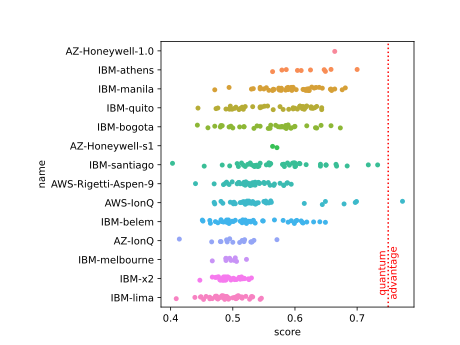
\includegraphics[width=1.1\colwidth]{nisq_stripplot.pdf}
  \end{figure*}
\vspace{10mm}
    \heading{$p$-value of uniformity test for 1000 shot runs}
    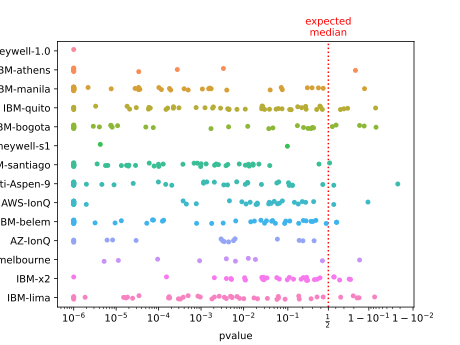
\includegraphics[width=\colwidth]{nisq_pvalue_logit.pdf}

\vspace{25mm}
\noindent
    \heading{Success rate vs. $p$-value}
    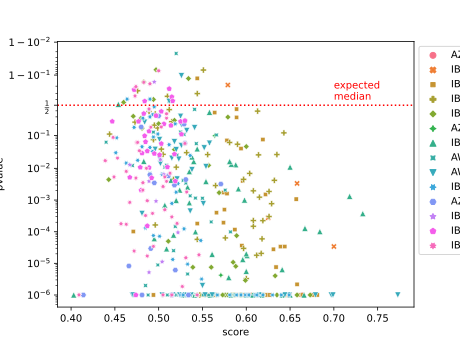
\includegraphics[width=\colwidth]{nisq_scatter.pdf}
    \end{center}

  \end{block}


\end{column}

\separatorcolumn

\begin{column}{\circwidth}
  \begin{block}{QNR17 test}
    \begin{center}
    \includegraphics[width=\circwidth]{V4_qnr17_nn.pdf}
    \vspace{10mm}
    \noindent

    \url{tinyurl.com/yckbk69n}
  \includegraphics[width=\circwidth]{QIP2022_QR.png}
  \end{center}

  \end{block}
  
\end{column}

\separatorcolumn
\end{columns}
\end{frame}

\end{document}
